\documentclass[preprint,12pt,times]{elsarticle}
%% Use the option review to obtain double line spacing
%% \documentclass[preprint,review,12pt]{elsarticle}

%% Use the options for a journal layout:
%%\documentclass[final,1p,times]{elsarticle}

%% The graphicx package provides the includegraphics command.
\usepackage{graphicx}
%% The amssymb package provides various useful mathematical symbols
\usepackage{amssymb}
%% The amsthm package provides extended theorem environments
%% \usepackage{amsthm}
%% The lineno packages adds line numbers. Start line numbering with
\usepackage{lineno}
\usepackage{cleveref}
\usepackage{usercommands}
\setlength{\parindent}{0pt}
\setlength{\parskip}{3pt plus1pt minus1pt}

\journal{Energy}

\begin{document}

\begin{frontmatter}

%% Title, authors and addresses

\title{A new methodology to compute the Exergy Cost}

\author{C\'esar Torres Cuadra}

\address{University of Zaragoza, Spain}

\begin{abstract}
The Exergy Cost theory was proposed in 1986,  by Valero et al., in the paper “General theory of energy saving”. This theory has been recognized as a powerful tool in the analysis of energy systems, and it has been applied to the assessment of alternatives for energy saving, local optimization, and thermoeconomic diagnosis.
The paper introduces a new methodology, based on productive linear models, which provides new and more efficient algorithms to determine exergy costs and to analyse the cost formation process of products and wastes. This methodology consolidates the mathematical foundations of the Exergy Cost theory and enhances the computer implementation of the thermoeconomic model.
The keystone of this new approach is the Stream-Flow-Process table, which describes the relationship “Processes uses flows to produce flows”, and characterizes the productive and dissipative structures of an energy system. 
\end{abstract}

\begin{keyword}
Exergy Cost Theory \sep Thermoeconomics \sep Productive models
\end{keyword}

\end{frontmatter}
%%\linenumbers activation

%% main text
\section{Introduction}
\label{S:1}
According to the management theory, cost is defined as the amount of resources required to produce something or deliver a service. Energy cost accounting, in addition to a managerial technique for measure the consumption of energy resources, must provide a rational method for assessing the production costs and their impact on the environment.
There is a wide international consensus that exergy is the adequate thermodynamic property to use for cost assessment, at least for energy systems. Thermoeconomics combines economics and Second Law analysis applying the economic cost concept to exergy.

The problem of exergy costs allocation was formulated \cite{Valero1986,ECT93} as follows: Given a system whose boundaries and level of aggregation that specifies the processes, which constitute it, have been defined. How to obtain the costs of all flows (energy carriers) that becomes interrelated in this structure?

Four conditions must be taken into consideration to solve this problem:
\begin{enumerate}
	\item The defined boundaries are relatives to the system under study. Energy, raw materials and economic resources used by the system must be specified.
	\item The level of aggregation provides a decomposition of the total irreversibility of the system among its processes or components. The level of aggregation chosen will affect the conclusions of the analysis. In fact, we do not have more information about the system than that defined by its aggregation level. The analyst should to disaggregate the system into processes and flows until the information could be used effectively. 
	\item The efficiency, as an indicator of process quality, must be used as physical criteria to allocate exergy costs. The exergy costs of resources used by a process must be allocated to their products proportionally to its exergy content. 
	\item The system produces undesirable flows or wastes, and consumes external resources to produce and eliminate these wastes. The formation process of wastes must be analysed, in order to determine the origin of waste flows and to make a correct cost allocation. 
\end{enumerate}

The Exergy Cost Theory \cite{ECT93} (hereinafter ECT) provides rational and objective criteria to allocate cost based on the definition of efficiency of the processes which constitute the system. It has been recognized as a powerful tool in the analysis of energy systems, and it has been applied to the assessment of alternatives for energy saving, local optimization, and thermoeconomic diagnosis.

The algebraic method provided by ECT to calculate exergy costs has some drawbacks: From the mathematical viewpoint, the original ECT approach does not ensure the existence, uniqueness and positiveness of the solution. From software implementation viewpoint, the method has limitations and accuracy problems when deals with complex structures. Finally, The problem of waste cost allocation is not treated in a rigorous and general way.

The aim of this paper is to introduce a new methodology to compute exergy costs, which combines graph theory an linear models with the allocation rules of exergy cost. This methodology will provide a rigorous mathematical approach that gives solutions to the cost allocation problem formulated above.

An energy system is defined beforehand as a set of subsystems or thermodynamic processes linked to each other and to the environment by another set of mass, heat, and work flows, quantified by its exergies. In essence, it constitutes a flowsheet, as it is shown in \cref{fig1}. This example represents a gas turbine cycle (henceforth called TGAS) that uses natural gas (flow \#5) to produces 10 MW of electric power (flow \# 6) and evaporates 8 kg/s of water at 20 bar of pressure, partially recovering the residual heat of gases. The exergy flow \#8 is calculated as the difference between the exergy of the saturated steam and and the inlet water. Finally, the waste combustion gases are expelled through a stack (flow \#9). This flowsheet indicates also the system boundaries and the aggregation level. The exergy values of the plant flows are show in \cref{tab4}.  

\begin{figure}[h]
	\centering
	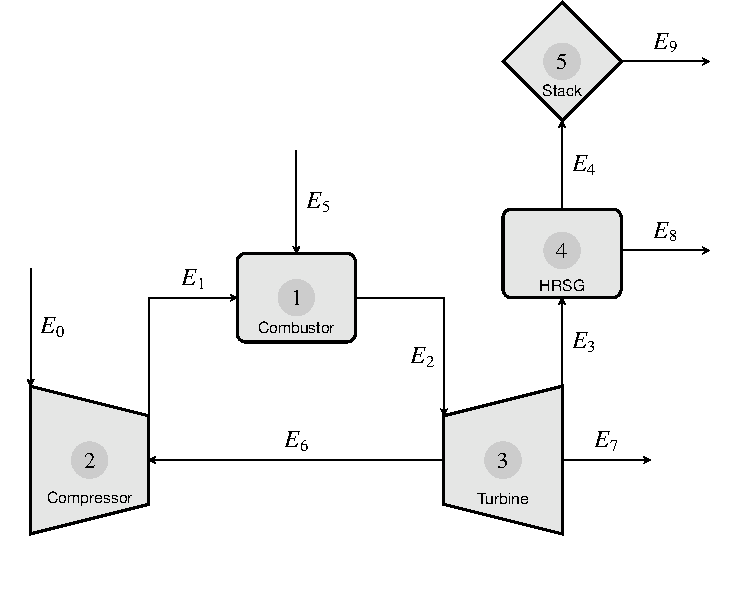
\includegraphics[width=0.65\linewidth]{tgas.pdf}
	\caption{Flowstream of TGAS plant}
	\label{fig1}
\end{figure}
\section{The Productive Structure}
\label{S:2}
Industrial installations have a productive purpose. Their objective is to obtain one or several products by processing external resources. For each process of the system is necessary to identify the flow that constitute their product streams, and the flow  required to obtain them, called fuel streams \cite{Tsatsaronis1985,SPECO06}. Energy flows (e.g heat or work) appear at the process inlet as fuel streams, or at the process outlet as product streams. When working with mass streams, it is appropriate to operate with exergy differences associated with each energy transfer between inlet and outlet.

A fuel stream will consist of:
\begin{itemize}
	\item One or several inflows that provide exergy to the process.
	\item Input and output flows belong to a mass flow stream that entering the process and leave it after transfer exergy to the process.
\end{itemize}
A product stream will consist of:
\begin{itemize}
	\item One or several outflows produced by the process.
	\item Output and input flows belong to a mass flow stream that entering the process and leave it after increasing it exergy.
\end{itemize}

The exergetic efficiency of a process $u$ is defined as the ratio between the exergy obtained or product and the exergy supplied or fuel. It measures how reversible a process is. The inverse value is the exergy unit consumption, i.e, the amount of resources required per unit of product obtained:
\begin{equation}
k_u=\frac{F_u}{P_u} \ge 1
\end{equation}
where $F_u$ is the exergy provided by its fuel streams and $P_u$ is the exergy of its product streams. The second law states that the exergy of the fuels is bigger than the exergy of the products, and the difference is the irreversibility $I_u$ of the process.
\begin{equation}
\label{eq:fpi}
F_u - P_u = I_u \ge 0
\end{equation}

%% The Appendices part is started with the command \appendix;
%% appendix sections are then done as normal sections
\appendix
\section{M-Matrices}
\label{A:1}
Very often problems in the biological, physical and social sciences can be reduced to problems involving matrices which, due to certain constraints, have some special structure. One of the most common situation is where a square matrix has non-positive off-diagonal and positive diagonal entries \cite{Smith:2012qr}. Such matrices appears, for example, in input-output production models in economics.

A square matrix \vm{A} is said to be \emph{diagonal dominant} if for every row of the matrix, the magnitude of the diagonal entry in a row is larger or equal than the sum of the off-diagonal entries
\[ \left|a_{ii}\right| \geq \sum_{i \neq j} {\left|a_{ij}\right|}
\qquad 1 \leq i \leq n \]
and it is called \emph{strictly} diagonal dominant if it at least exists a row $i_0$
so that: $\sum_{j}{\left| a_{i_0 j} \right|} > 0$

A matrix \vm{A} is said positive if all its elements $a_{ij}\ge0$, and at least one element is bigger than zero. 

A positive matrix \vm{B} is called \emph{productive} \cite{Smith:2013jd} if there is a vector $\vm{x}_0$ so that
$\vm{B}\,\vm{x}_0 < \vm{x}_0$

Let $\lambda _{1},\ldots ,\lambda _{n}$ be the (real or complex) eigenvalues of a matrix \vm{B}. Then its spectral radius $\rho(\vm{B})$ is defined as:
\(\displaystyle \rho (\vm{B})=\max \left\{|\lambda _{1}|,\ldots ,|\lambda _{n}|\right\}.\)

Consider the matrix $\vm{A}=\mdiag{U}-\vm{B}$, and $\vm{B}>0$. The matrix \vm{A} is said an M-matrix, if it satisfy one of the following equivalent properties:
\begin{enumerate}
	\item \vm{B} is productive.
	\item $\rho(\vm{B})<1$.
	\item There exist a positive diagonal matrix \vm{D}, such $\minv{D}\vm{A}\vm{D}$ is strictly diagonal dominant.
	\item \vm{A} has inverse and \minv{A} is positive.
	\item $\displaystyle{\lim_{k\rightarrow\infty}\vm{B}^k=0}$, and 
	$\minv{A}=\vm{U}+\displaystyle{\sum_{k=1}^{\infty}{\vm{B}^{k}}}$	
\end{enumerate}	
M-matrices has also important properties in relation with numerical analysis. In particular, the LU factorization of an M-matrix is guaranteed to exist and can be stably computed without need for numerical pivoting. \cite{Smith:2012qr}

%% References with bibTeX database:
\section*{References}
\bibliographystyle{model1-num-names}
\bibliography{sample}
\end{document}